\documentclass{standalone}
\usepackage{tikz}

\begin{document}
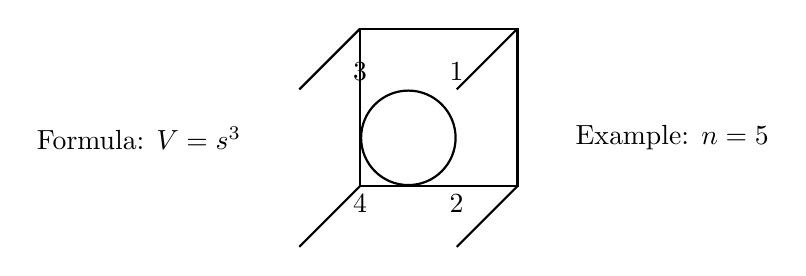
\begin{tikzpicture}[scale=2]
    % Draw the cube
    \draw[thick] (0,0,0) -- (1,0,0) -- (1,1,0) -- (0,1,0) -- cycle;
    \draw[thick] (0,0,0) -- (0,0,1);
    \draw[thick] (1,0,0) -- (1,0,1);
    \draw[thick] (0,1,0) -- (0,1,1);
    \draw[thick] (1,1,0) -- (1,1,1);

    % Draw the circle
    \draw[black, thick, fill=white] (0.5,0.5,0.5) circle (0.3);

    % Label the coordinates
    \node[above right] at (0.7,0.8,0.5) {1};
    \node[below right] at (0.7,0.2,0.5) {2};
    \node[above left] at (0.3,0.8,0.5) {3};
    \node[below left] at (0.3,0.2,0.5) {4};

    % Add other symbols and numbers outside the circle
    \node[right] at (1.5,0.5,0.5) {Example: $n = 5$};
    \node[left] at (-0.5,0.5,0.5) {Formula: $V = s^3$};
\end{tikzpicture}
\end{document}